\chapter[Results]{Results}
% Per research question a section is dedicated, describing the results. The final critical walkability factors are given in section \ref{Rrq1}
% The average walking speed of elderly can be found in \ref{Rrq1b} . 
% Section \ref{rq2a} shows the data collection and pre-processing steps for the analysis of existing geo-data. The GBKA an the AHN are used.
% In section \ref{rq2b} the data collection and pre-processing steps for the collection of our own geo data, with GPS devices and an accelerometer. Eventually, the steps for analysing this data is explained in the last part of this section.
% The methods for combining the existing geo-data with the own collected data is explained in section \ref{rq2c}. With a Change Point detection algorithm, changes in the time series of the rollator walks are found, and plotted on the map to compare it to other data sources. 
% RQ1 
\section{Results RQ 1. - Finding the critical factors for walkability}
\subsection{Findings critical factors from literature}
Table \ref{literature} shows a summary of the occurrence of the amount a certain criteria is found in literature, per category and level. The criteria are counted double if found multiple in different literature pieces. As can be seen in the table, most reports mentioned criteria that can be found on pavement level and criteria falling into the category of route attractiveness. \newline

\begin{table}[H]
\centering
\caption{Overview of finding in literature research \label{literature}}
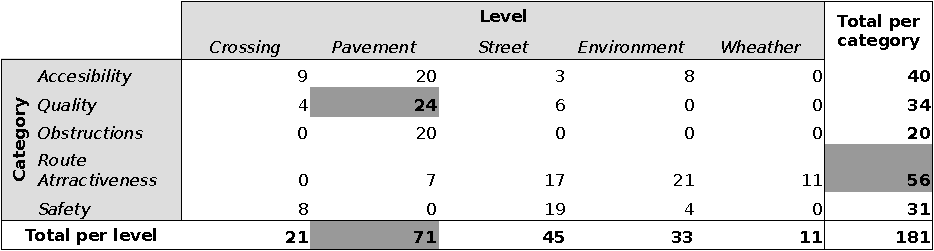
\includegraphics[width=\textwidth]{img/R_Final_overview_literature_summary.pdf}
\end{table}

In the next table, a more detailed overview of the criteria found on pavement level is given. For criteria about the pavement and objects in the way, even a more detailed criteria list is given and the amount of literature studies mentioning them. Two criteria are mentioned most, irregular surfaces and (wrongly) parked bikes and cars. 
\clearpage

\begin{table}[tp]
\centering
\caption{Detailed overview of criteria at pavement level \label{literaturepavement}}
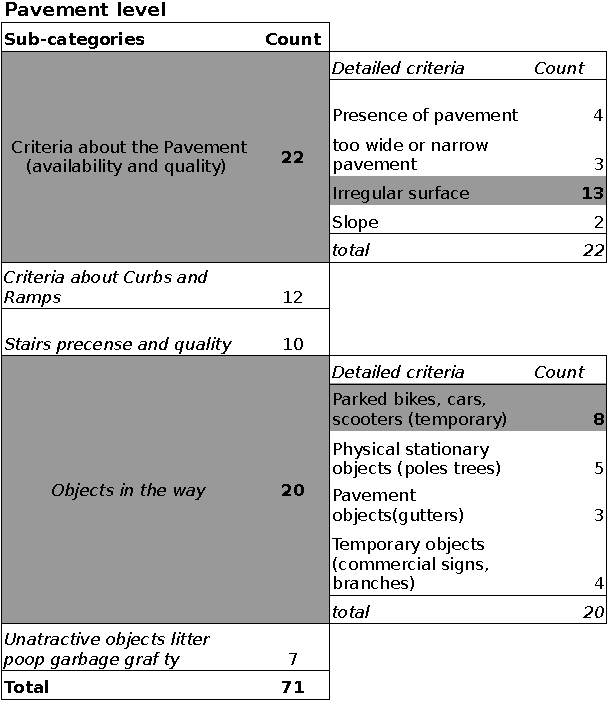
\includegraphics[width=0.75\textwidth]{img/R_Final_overview_literature_pavement.pdf}
\end{table}


% %Pavement suitability

% This will include the availability of a pavement, the minimum width, the surface material, the presence of curbs and ramps, slope.
% Standard pavement should be $1.2m$, excluding the curb. In intensively used pavement, around schools, shops etc., the width should be around $1.8m$. Narrow pavements are $0.9m$, excluding curb.  Verschuur

% Verschuur already did a study on these factors defining

% is information a classification can be made on the pavements on how suitable they are, like Verschuur:
% All pavements with a with smaller than 1.2 m are assigned as not suitable. All pavements in intensively used areas, smaller then 1.8m are also assigned not suitable. 
% All pavements wider or equal to 1.2 in standard areas are positive
% All pavements wider or equal to 1.8 in intensively used areas are positive.
% All pavements wider or equal to 1.8 in standard areas are very positive.
% As an example, Figure 6 shows a map from Verschuur on pavement width analysis in combination with presence of barriers. 

% Figure 6 Example pavement suitability from (Verschuur, 2014


% Positive objects
% Route attractiveness
% land use mix
% Overall street suitability and environmental influences
% Street connectivity
% Traffic density
% Pavement density


\clearpage

\subsection{Summary personal interviews}

\textbf{Participant 1.}
Uses a wheeled walker already for 8 years. Without she loses balance, really depended on the rollator. Though short distances often without, but would be safer with. Although she has severe fright of falling, she walks outside at least once a day, half an hour. This to stay fit, but she would rather stay at home. When she gets tired, her ankles weaken and she is even more afraid of falling. 
For her, if the pavements would be more smooth, I would be able to walk much further because it is more easy and she would not get tired that quickly. Loose tiles, pits, wrongly parked cars, tourists, sloping pavements are a problem to her. Especially the amount of people on the street, she tries to avoid. 
In conclusion, walking is not a relaxing activity for her, she goes out, because she wants to move to stay fit. Smooth surface to walk on would increase her ability to walk and she would be able to walk more easily and further. The business on the streets is not her thing and the purposely avoids this. 

\textbf{Participant 2. }
Participant 2 is a real outdoor walker. She goes out on the streets several times a day and strolls around the whole neighbourhood. She uses the rollator for .. years and feels that the rollator is really easy and a blessing for her. It keeps her mobile and enjoy Amsterdam around her. 
Problems mentioned by her are the uneven tiles or half loose tiles. So not well maintained pavements. Also when cars are parked wrongly and this makes her move off the high curbs is difficult. 
She mentioned that the resting benches are way too low. So if she would sit on these she has difficulty getting up again. 
She was really positive about the people on the street, in her perception they are friendly and helpful. Also she attached a bell on her rollator, so that if someone is in the way she would just ring the bell and she can pass. 

\textbf{Conclusion.} Most often named: 
\begin{itemize}
\item Irregular surfaces as in Loose tiles or bad maintenance. 
\item Sloping surfaces
\item Wrongly parked cars
\end{itemize}


\subsection{Summary interviews at Rollator Loop}
The age of the participants ranged from 77 to 94. Some used the rollator for more than 6 years, while others only since half a year. When starting using a rollator, participants said they did not dare to walk without it any more, because of fear of falling. Most of them mentioned grocery shopping as the main activity for using a rollator outdoors.
Noticing the bad quality of the streets only occurs to you when your mobility worsens and you start needing a rollator to help you. 
Problems mentioned were; roots of trees make the pavement uneven, pavements are convex and these sloping circumstances need you to adjust the rollator all the time. The maintenance is not sufficient. Not nicely finished pavements, transition from tiles to asphalt not even. Public transport stops not adjusted. Tram rails. 
On the positive side, there is enough space to walk. Not all participants have difficulty with going on and off the pavement. 
One participant did not have any problems while walking on the street while walking to the grocery store across the street a few times per week. 
Sloping pavements and bad maintenance as in uneven surface, were mentioned several times. 

\subsection{Findings Amsterdam policy and summary interview municipality}
More post placed and raised pavements, to avoid cars on the pavement.
Public transport stops are raised for easier entrance into the bus and trams. 
Puccini method as design policy for public space. 
GIS data available but not sure what. 
Centre, tourist are the main problem. 
More ageing. Accessibility is getting a problem. Living independent is policy. There is still a lack at the municipality in providing facilities and care. 
Mostly focus on accessibility of public transport and public buildings. 
More people walk. 
Putting up a new framework for pedestrians. First stage to be completed end of 2015. The framework includes the design policy for public space with design principals, assumptions, guidelines, goals, tests, and products. 
Integrated pedestrian policy, covering all from crowd management to accessibility. 
Indicators should be, measurable so quantitative but also qualitative.
Goal is to grow, more space for pedestrians, more use of the public space.
Before the policy was scattered, now focus on one pedestrian policy. 


%Amsterdam policy
The Puccini Method states that the side-walks are often the residual area that remains after the design of the road. \cite{puccini2014}

Altijd een minimale vrije doorgangsbreedte noodzakelijk van 1,50 meter;
- In door voetgangers druk gebruikte stadsstraten een minimale vrije doorgangsbreedte
noodzakelijk van 2,50 meter.
14In de praktijk is er veel extra ruimte nodig om alle meubilair en objecten te plaatsen. Zodoende moet
er bij de minimale breedtes:
- 0,5 meter extra worden opgesteld ten behoeve van een ‘slimme strook’ waarin
parkeermeters, lantarenpalen, banken, papierbakken etc. kunnen worden opgenomen;
- Indien nodig één meter extra worden opgeteld ten behoeve van uitstallingen van winkels
aan de gevelzijde;
- Indien nodig 1,80 meter extra worden opgeteld indien er fietsenrekken op het trottoir
staan.



Trottoirbreedte en -helling
Voor voetgangers, gehandicapten, met name rolstoelers en lopende gehandicapten met
begeleider geldt een gewenste obstakelvrije loopruimte van 2,00m (op grond van landelijke
norm minimaal 1,80m).
De gewenste maat is verder afhankelijk van de intensiteiten, functies, etc 1 .
Naast deze maat dient rekening te worden gehouden met extra ruimte van circa 1,00m
(minimaal 0,75m) aan beide zijden van het trottoir ten behoeve van objecten zoals verkeers-
borden, brandweerkranen, elektriciteitskasten, lantaarnpalen, reclame- en informatiezuilen,
hekken, planten, geparkeerde fietsen, etc. De extra trottoirbreedte moet voldoende zijn om de
vrije loopruimte van minimaal 1,50m te waarborgen.
De toe te passen helling mag met het oog op gebruik door gehandicapten niet steiler zijn dan
1: 25 (4%). Bij grote hoogteverschillen zijn liften gewenst.
Voor een boomstrook op het trottoir dient minimaal 2,00m aangehouden te worden. Deze
strook kan dan tevens gebruikt worden voor het plaatsen van diverse objecten en straatmeubi-
lair, maar ook voor inpassing van laad- en loshavens of parkeervakken.~\cite{leidraad2011}

\subsection{Final list critical factors}

The top 3 critical factors derived from all of the above are: 
\begin{enumerate}
\item Wrongly parked bikes and cars
\item Sloping pavement
\item Irregular pavement
\end{enumerate}

The first item will not be examined, for parked bikes and cars are temporary obstacles which can be hard to detect through stationary geo data. The applicability of Geo information systems for monitoring wrongly parked bikes and cars is a whole new study on its own.

The sloping pavements will be examined with available height data(AHN2). The irregular pavement will be examined trough accelerometer measurements of the rollator movements. 

\clearpage

\subsection{Average walking speed}
The average walking speed found was 4.62$km/h$. In the table \ref{statistiswalkingspeed} and figure \ref{averagewalkingspeed}, clearly can be seen that the average walking speed decreases when walking longer distances. 
The total number contains all participants labelled as male, female or unknown. Therefore, the sum of male and female differences from the total number.

\begin{figure}[h]
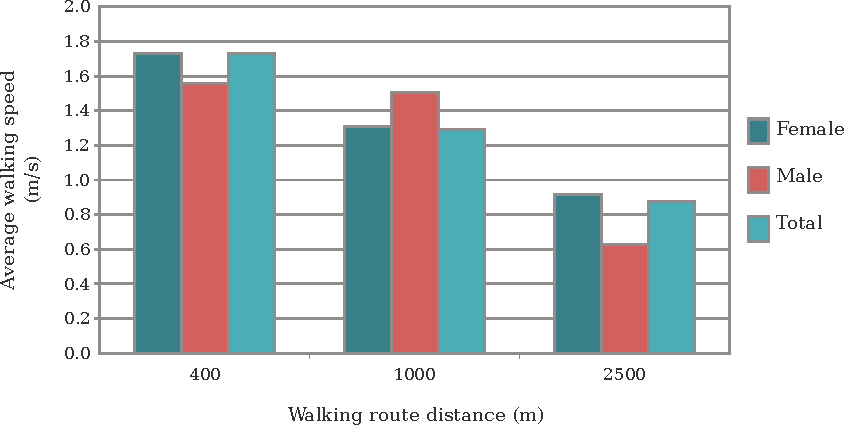
\includegraphics[width=\textwidth]{img/R_averageWalkingSpeed.pdf}
\centering
\caption{Average waling speed, participants Rollator loop 2014 and 2015 \label{averagewalkingspeed}}
\end{figure}


\begin{table}[h]
\caption{Average walking speed, participants Rollator loop 2014 and 2015 \label{statistiswalkingspeed}}
\centering
\begin{tabular}{|p{70pt}|p{70pt}|p{70pt}|p{70pt}|p{70pt}|}
\hline
Distance & Sex & Count & $m/s$ & $km/h$ \\
\hline
400 & Male	 & 25	& 1.56 & 5.60 \\
400 & Female & 97	& 1.73 & 6.23 \\
% 400 & Total	 & 134  & 1.73 & 6.23 \\
\hline
1000 & Male		& 5	 & 1.51	 & 5.42\\
1000 & Female	& 28 & 	1.31 & 4.72\\
% 1000 & Total	& 37 & 	1.29 & 4.65\\
\hline
2500 & Male		& 1	 & 0.63	 & 2.26\\
2500 & Female	& 7	 & 0.91	 & 3.29\\
% 2500 & Total	& 8	 & 0.88	 & 3.16\\
\hline
& Total & 179 & 1.30 & 4.62 \\
\hline
\end{tabular}
\end{table}
\clearpage

%RQ2a

\section{Results RQ 2A -  Collection and analysis of available geodata}
\subsection{Determining pedestrian area with the GBKA}
The GBKA was used to determine how much surface is determined for pedestrians. In annex \ref{Ajordaan} the total area of the Jordaan is shown. Here, some detailed maps shows some areas where the classification turned out to be okay, but also contains some streets which area wrongly assigned pedestrian area. In total the Jordaan has around 300000$m^2$ of public road surfaces. About 53\% of this is intended for pedestrians according to the developed approach. This share of road does contain poles, lanterns, bicycle racks, parking plots and all other street furniture. 

\begin{table}[h]
\caption{Statistics pedestrian area \label{statroadsections}}
\centering
\begin{tabular}{|l|l|l|}
\hline
Road Section & Total Area	& Percentage\\
\hline
All Road Sections & 293317.25 & 100.00\\
\hline
1. Transport & 133789.66 & 45.61\\
2. Pedestrians & 156159.49 & 53.24\\
3. Unpaved	& 3368.1 & 1.15\\
\hline
Below 4\% slope & 114341.08 & 38.98\\
Pedestrian below 4\% slope & 24466.67 & 8.34\\
\hline
\end{tabular}
\end{table}

Figure \ref{jordaanroad} shows in white, the pedestrian area as approached. The Tweede Boomdwarsstraat is wrongly classified. Also bridges are mostly wrongly classified. The parking plots in the centre of the road Westerstraat are classified as pedestrian area but are not suitable for pedestrians, as it is full with cars and other street furniture. See Figure \ref{westerstraat} image from Google street view of the Westerstraat. 

\begin{figure}[h]
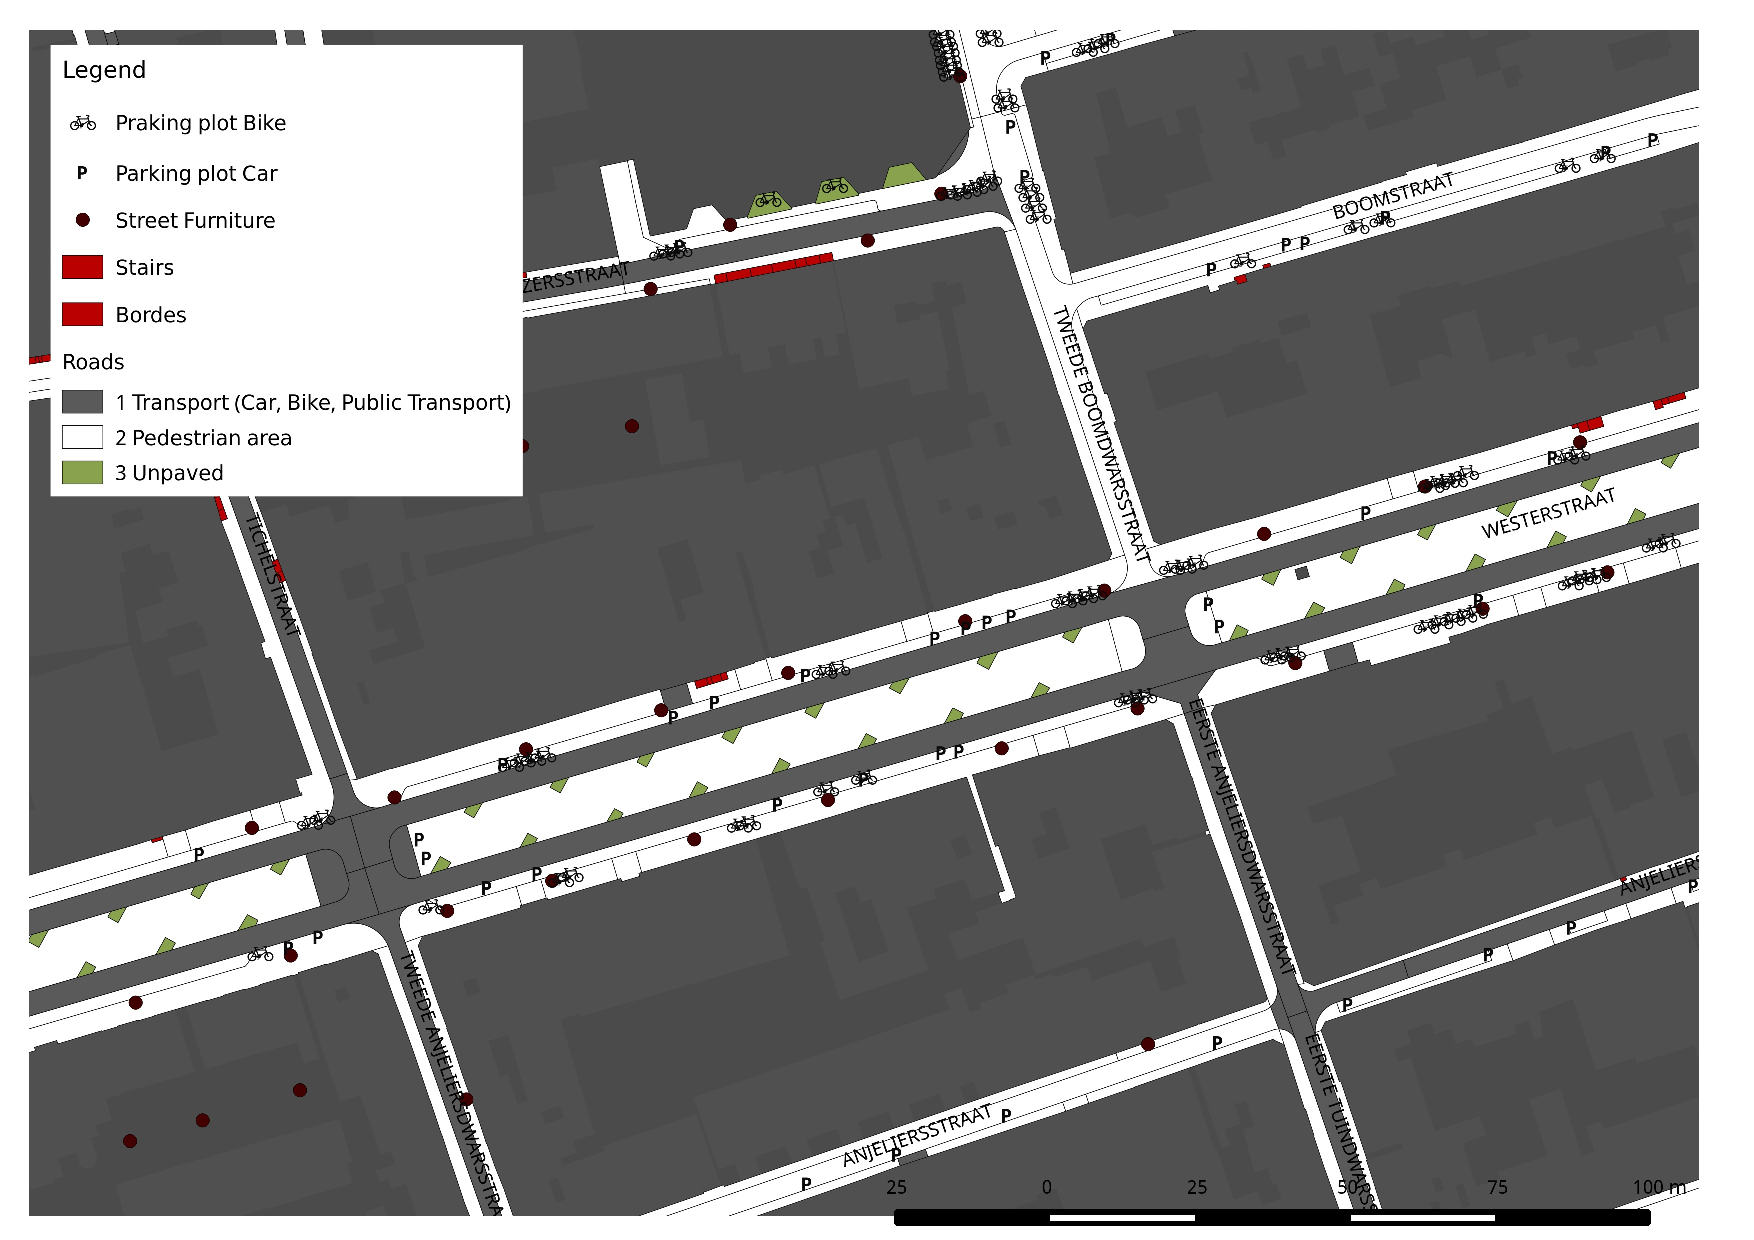
\includegraphics[width=\textwidth]{img/R_Jordaan_weg_detail_resultat.pdf}
\centering
\caption{
Detail Jordaan Road Section classification\label{jordaanroad}}
\end{figure} 

\begin{figure}[h]
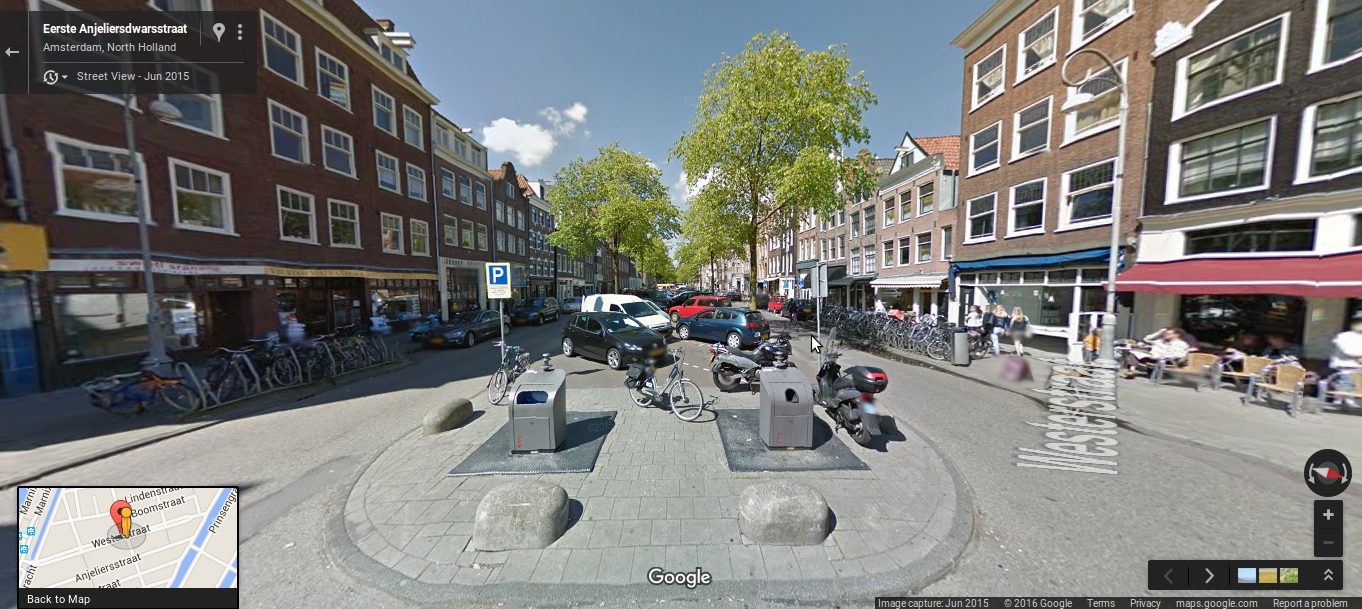
\includegraphics[width=\textwidth]{img/R_Westerstraat.png}
\centering
\caption{
Google Street View image of the Westerstraat\label{westerstraat}}
\end{figure} 


\clearpage

\subsection{Mapping sloping surfaces with AHN data}
In table \ref{statroadsections} from the previous section, also the area pedestrian area below 4\% of slope and the total area below 4\%slope is given. Consecutively, 8\% and 39\% of the total area.
In figure \ref{jordaanslope} the Westerstraat can be seen, with the slope below 4\% in green. The roads destined for cars are shown more general green except for the speed bumps which can be clearly distinguished. The pedestrian area on the other hand, shows more red spots. When looking at the average slope per road section polygon, also the car area (1.) stays below the 4\% while the pedestrian area has higher slopes. Figure \ref{jordaanroadslope}.
The original hight map of the AHN2 can be found in Annex \ref{AAHN}.
\begin{figure}[h]
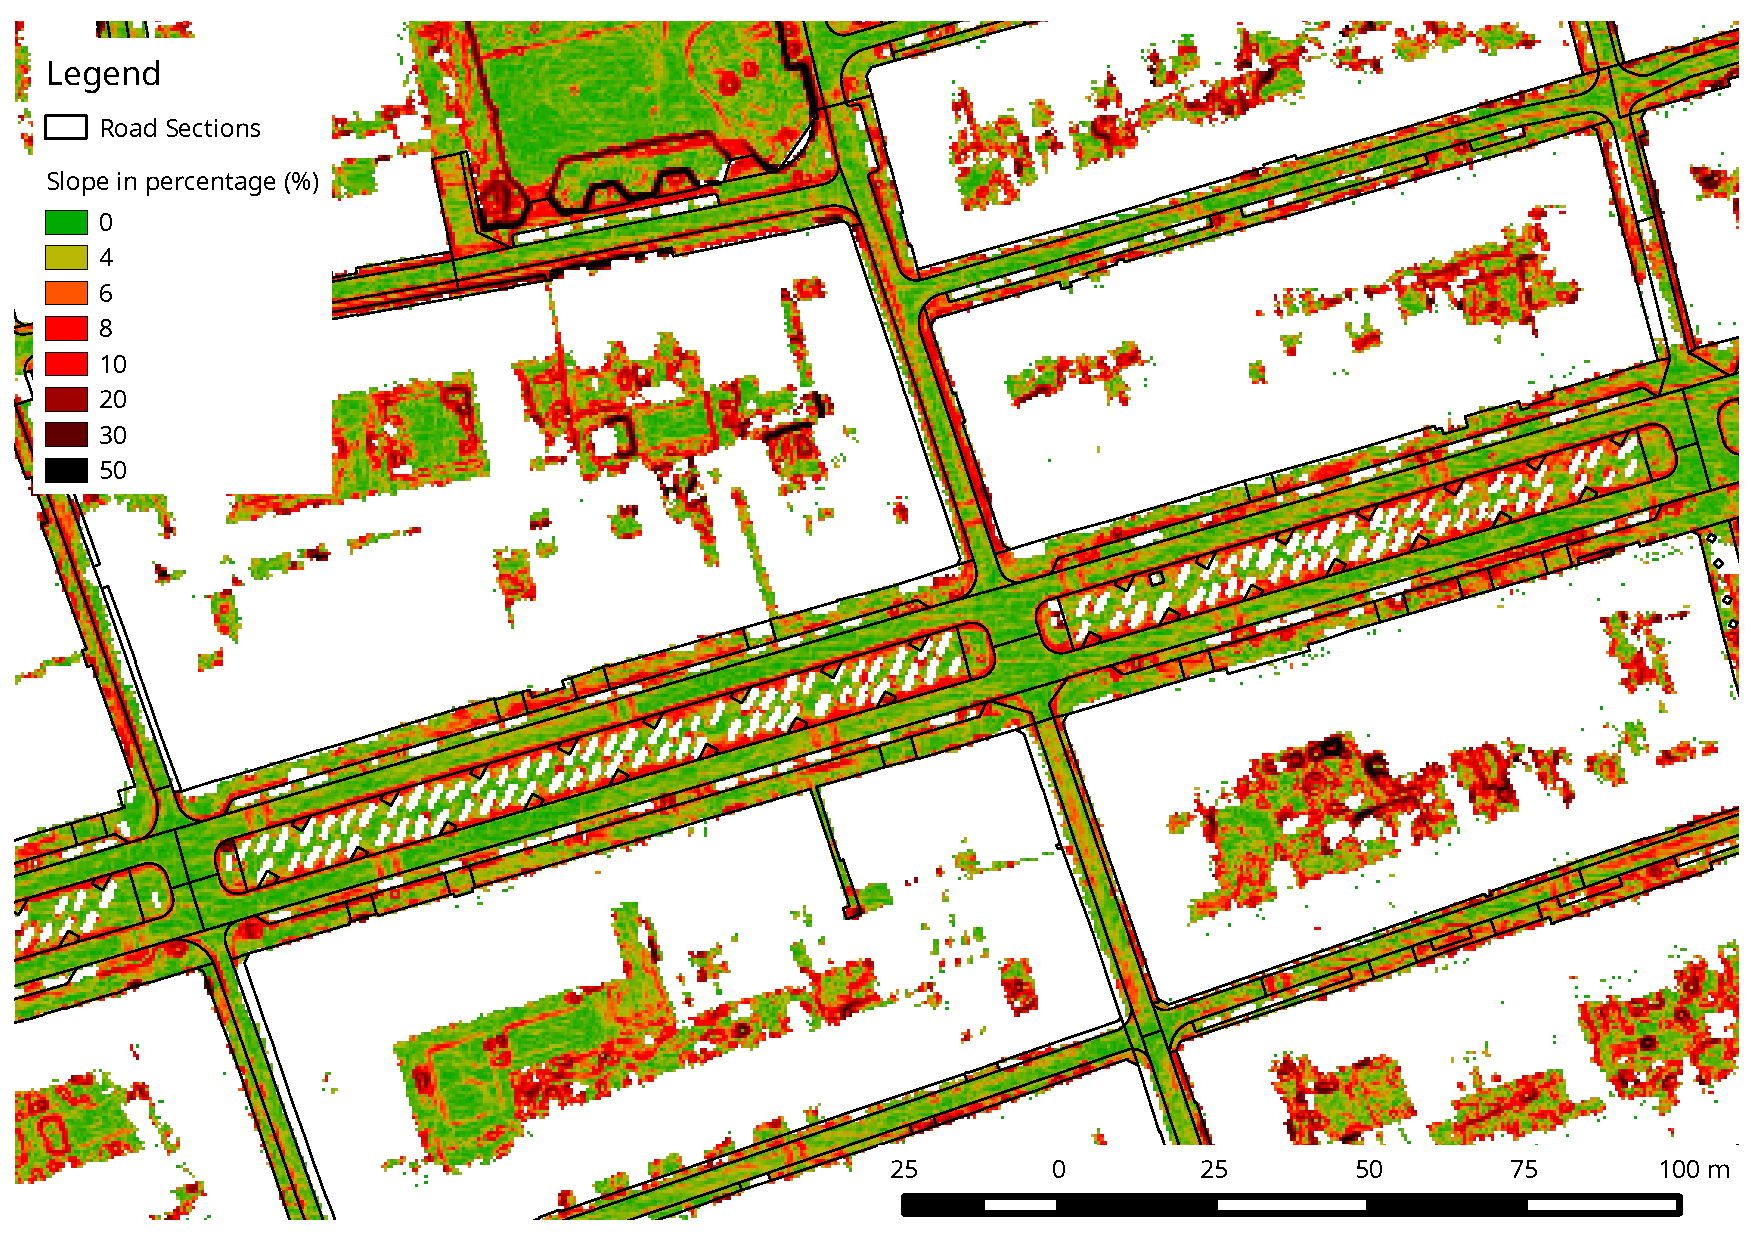
\includegraphics[width=\textwidth]{img/R_slope_jordaan.pdf}
\centering
\caption{
Detail Jordaan Slope map\label{jordaanslope}}
\end{figure} 

\begin{figure}[h]
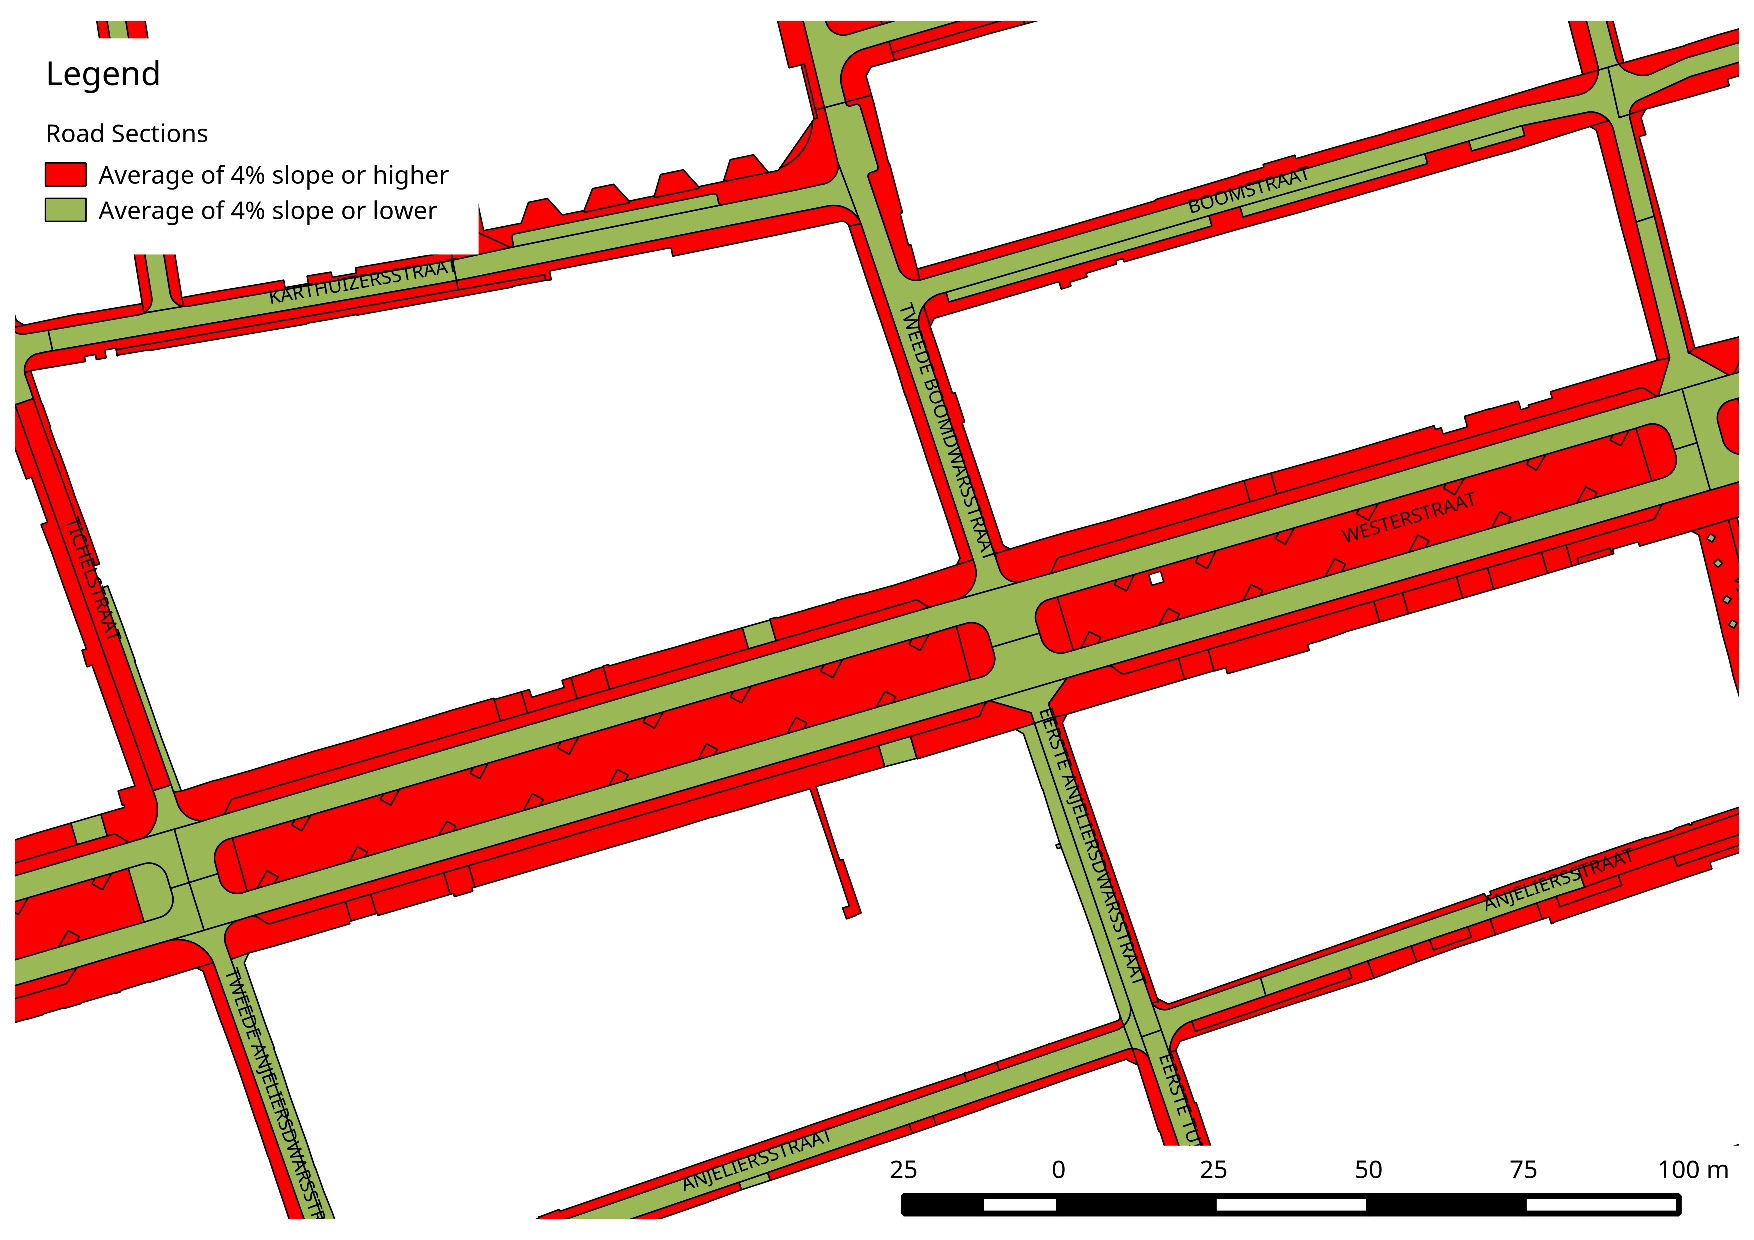
\includegraphics[width=\textwidth]{img/R_averageslope_jordaan_roadsection.pdf}
\centering
\caption{
Detail Jordaan Average Slope per road section\label{jordaanroadslope}}
\end{figure} 
\clearpage



\section{Results RQ 2B- Collection of geodata of rollator movements and analysis
}
\subsection{Mapping irregular surfaces with an Accelerometer}

Figure \ref{figsurfaces} shows the accelerometer output of the z-axis per measured surface. The exact statistical summary of every surface is given in table \ref{surfacehindrance}. Containing the total acceleration mean, standard deviation, the variance, the minimum and maximum, first and third quantile and the median. The median and mean are roughly the same for every surface, because the accelerometer measures acceleration in the vertical direction around 1$m/s/s$, which is equal to gravity. Any acceleration aiming up, will also go down. The extent of acceleration a surface causes in the vertical direction, or the standard deviation or variance, tells more about the differences in surface.
To show more visually the differences in variance per surface, the box plots \ref{boxhindrance} show spreading per surface. Clearly the difference per surface can be seen. The smooth concrete inside, gave almost no acceleration in the vertical direction, while stones or grass showed more vibration and so higher and lower values in minimum and maximum as well as the standard deviation and variance.   

% mss nog plaatje van de GPS tracks locaties en de gekoppelde data? 
\begin{figure}[H]
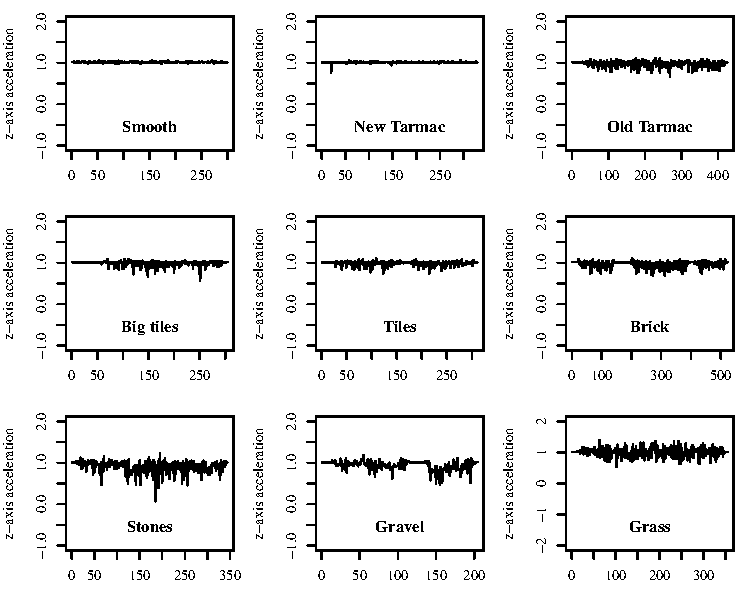
\includegraphics[width=\textwidth]{img/R_AllsurfaceGraphs.pdf}
\centering
\caption[Accelerometer data per surface]{
Accelerometer data per surface\label{figsurfaces}}
\end{figure} 

\begin{table}[ht]
\caption{Statistic summary surface hindrance \label{surfacehindrance}}
\centering
\begin{tabular}{|p{46pt}|p{30pt}|p{30pt}|p{30pt}|p{30pt}|p{30pt}|p{30pt}|p{30pt}|p{30pt}|}
\hline
Surface: & Mean & Std dev & Variance & Min & Q1 & Median & Max & Q3\\
\hline
Smooth & 1.02 & 0.02 & 0.00 & 0.97 & 1.02  & 1.06 & 1.01 & 1.03 \\
New tarmac  & 1.01  & 0.02  & 0.00  & 0.77  & 1.01  & 1.06 & 1.01  & 1.02\\
Old tarmac & 0.97 & 0.07 & 0.01 & 0.67 & 0.99 & 1.12 & 0.94 & 1.02\\
Big tiles & 0.99 & 0.07 & 0.00 & 0.58 & 1.01 & 1.10 & 0.98 & 1.02\\
Tiles & 0.99 & 0.06 & 0.00 & 0.74 & 1.01 & 1.10 & 0.97 & 1.02\\
Brick & 0.96 & 0.07 & 0.01 & 0.68 & 0.98 & 1.11 & 0.92 & 1.01\\
Stones & 0.91 & 0.14 & 0.02 & 0.07 & 0.94 & 1.23 & 0.84 & 1.01\\
Gravel & 0.94 & 0.12 & 0.02 & 0.48 & 0.97 & 1.19 & 0.87 & 1.01\\
Grass & 1.01 & 0.15 & 0.02 & 0.54 & 1.02 & 1.40 & 0.93 & 1.10\\
\hline
\end{tabular}
\end{table}

\begin{figure}[hb]
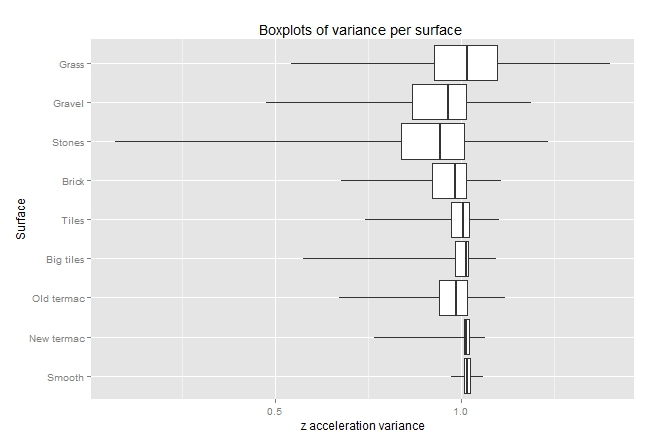
\includegraphics[width=\textwidth]{img/R_Surfaces_Variance.jpeg}
\centering
\caption{Box plot surface hindrance variance per surface \label{boxhindrance}}
\end{figure} 

% \begin{figure}[ht]
% 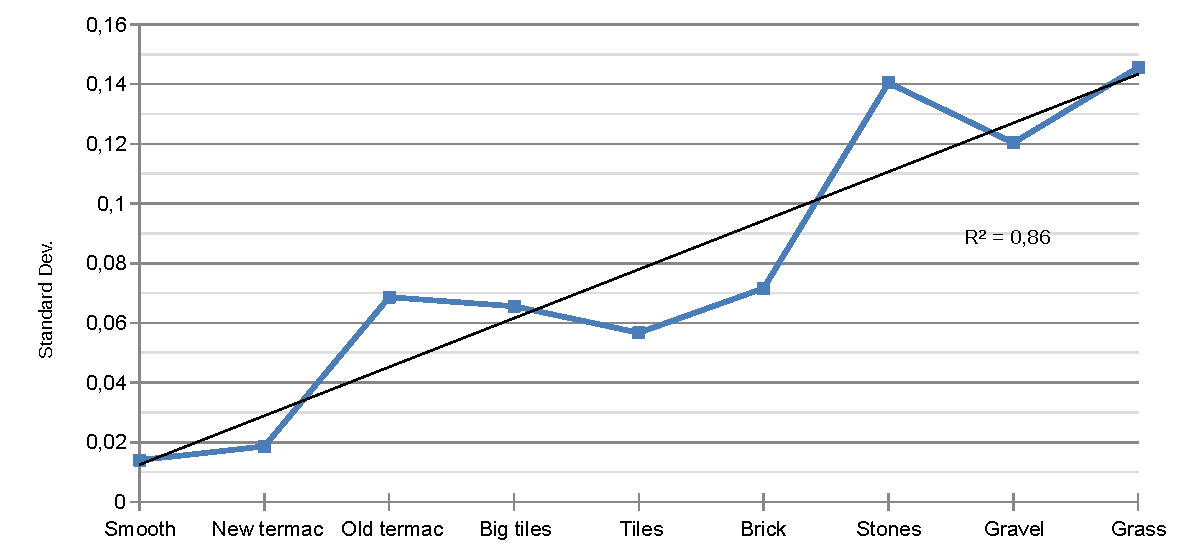
\includegraphics[width=\textwidth]{img/R_statistics_surfaces2.pdf}
% \centering
% \caption{The surface hindrance standard deviations with the regression line \label{hindrance2}}
% \end{figure} 
% \clearpage
\clearpage

\subsection{Comparison with Matthews et al. 2003}
From the standard deviation relative scores are assigned. Taking the smooth surfaces as basis value 1. The other values are calculated as a factor from this. Lower scores represent levels of least hindrance while higher scores represent high levels of vibration and so more hindrance. These factors are compared against the factors found in Matthews et al.(2003) and matched upon the surface description. The factors form Matthews do differ in value but are also calculated relatively to its most smooth surface, concrete. When plotting both values against each other a correlation coefficient of 0.72 is found. Indicating a positive and high correlation between the two data sets. 

\begin{table}[hb]
\caption[Relative scores of surface hindrance.]{Relative scores of surface hindrance. Measured and Matthews \label{compare}}
\centering
\begin{tabular}{|p{67.6pt}|p{55.6pt}|p{55.6pt}|p{55.6pt}|p{55.6pt}|p{55.6pt}|}
\hline
Surface & Standard Deviation of z-ax & Percentage & Factor & Factor given by Matthews & Surface name by Matthews \\
\hline
Smooth & 0.01 & 100.00 & 1.0 & 1 & Concrete \\
New tarmac & 0.02 & 132.72 & 1.3 & & \\
Old tarmac & 0.07 & 489.01 & 4.9 & 1.3 & Tarmac \\
Big tiles & 0.07 & 467.30 & 4.7 &  & \\
Tiles & 0.06 & 404.02 & 4.0 & 1.2 & Paving \\
Brick & 0.07 & 510.27 & 5.1 & 1.6 & Brick \\
Stones & 0.14 & 1000.62 & 10.0 & & \\
Gravel & 0.12 & 857.41 & 8.6 & 8 & Gravel \\
Grass & 0.15 & 1037.63 & 10.4 & 6 & Grass \\
\hline 
\end{tabular}
\end{table}

\begin{figure}[hb]
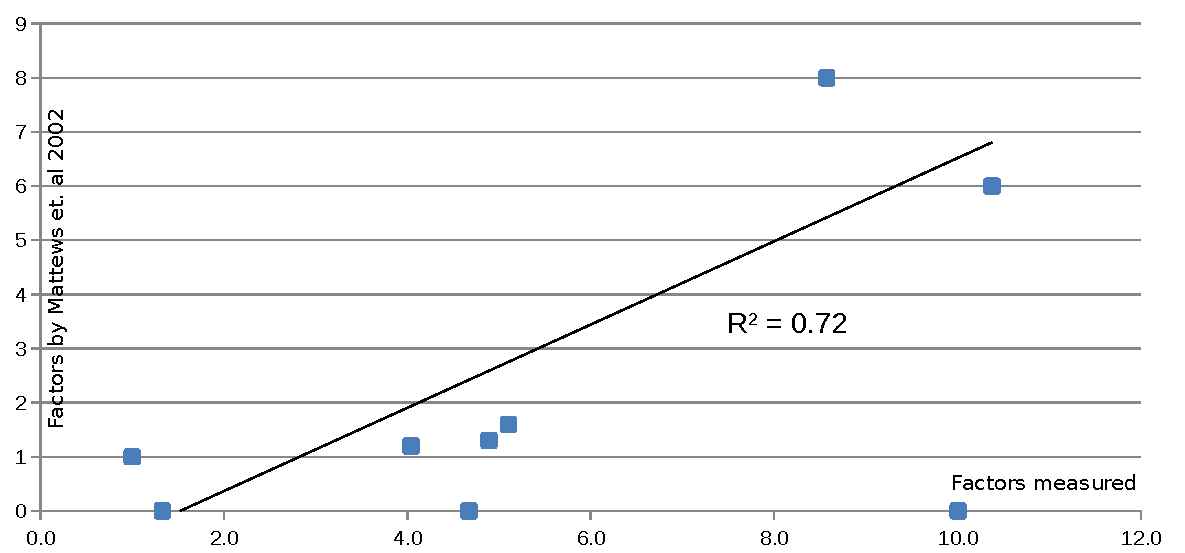
\includegraphics[width=\textwidth]{img/R_factors_compared.pdf}
\centering
\caption[Comparison factors measured and factors given]{
Comparison factors measured and factors given by Matthews et al. 2003\label{comparefig}}
\end{figure} 

\clearpage



\section{Results RQ 2C - Mapping abnormal or change events with Accelerometer, GPS and AHN2 data}

\subsection{Comparing different Change Point detection methods}

First the different changepoint detection methods and penalty values had to be tested to see which model approaches the most plausible result and approaches the truth the best. This was shortly done for all datasets, here we will show possibilities of the acceleration output of the $z-ax$ of the rollator route in detail. See figure \ref{cpcomp} Walking with a speed of around 4$km/h$, the distance between each measured point is  around 25$cm$ with a sample frequency of 5 points per second (Normal settings). The total route was 500 meter. 

The first method, finding change points for the variance with PELT method, resulted in 10 change points. So on average one change point per 100 meter. Some outlying peeks are missed by the model, and are not enclosed by changepoints, while they could indicate an unevenness in the surface. 

The second method variance with PELT $1.5*log(n)$ resulted in 69 points. On average one point per 7 meter. Now, the outlying peaks are enclosed by two changepoints, indicating exactly where a abnormality happens. Changing the penalty value solves the problem of over-fitting the model. The penalty increased the number of parameters in the model and almost always improves the goodness of fit. 


Method BinSeg and BinSeg $1.5*log(n)$ took a longer computing time and resulted in only 5 change points for the variance. Method PELT and PELT $1.5*log(n)$  for the mean resulted in no change points. Method SEGNeigh on the mean of the variance didn't gave any output. The PELT method for both the mean and variance at the same time had 50 change points.  


Eventually, for detecting changepoints in the variance of the acceleration the PELT method with a manual pen value of $1.5 * log(n)$ is used to overcome over and under fitting. For it showed the most plausible result.

A same kind of figure for the analysis of the best methods to detect changepoints in the speed dataset, can be found in annex \ref{Acptest}.
For the speed we look at changes in the mean.

Significant changes are, that the speed drops 2 times almost to the zero, the first drop is waling up and down the pavement curb. The second drop is a curve in the road where probably a short stop was made.

The first method, finding change points for the mean with PELT method, resulted in 3 change points and missed the second drop in speed.  The second method variance with PELT $1.5*log(n)$ resulted in more points and did detect the second drop in speed. Plus, broke up the first stop into 3 parts. Method BinSeg, BinSeg $1.5*log(n)$ and SEGNeigh resulted in no output.The PELT method for both the mean and variance at the same time had made a break point on every value of a change in speed, so over-fitted the model. 
When looking at the change points in the variance, PELT and PELT $1.5*log(n)$, more change points are detected, sometimes giving a logical breakpoint, for example at the huge drop in speed. But also multiple points really close to each other are detected, singling out steps in gradually decrease or increase in speed over a longer distance. Which gives too many points, as every 5 meter. 


For every individual dataset, the best possible penalty settings are considered, for there can be a big difference in characteristics of the dataset for speed, slope and acceleration. Though, for all datasets, the PELT method was used, because it has less computing time but has a good accuracy and distribution of change points over the dataset. In general the slope datasets resulted in too much over-fitting, therefore a different penalty type was chose, the AIC or the BIC model. For every dataset the model of fit is indicated in the summary tables of the next section.  





% ### Because of overfitting the model of speed a penatlyt type of BIC AIC or Hanan-Quinn can be chosen to solve the problem of overfitting.
% ##  a penalty term for the number of parameters in the model; the penalty term is larger in BIC than in AIC.
% ##he penalty discourages overfitting (increasing the number of parameters in the model almost always improves the goodness of the fit).
% ## we use an adjusted penalty to overcome the problem of overfitting. The GPS contains abonormal peaks due to measurement errors. If a model is generated that fits too well, these are taken as truth. Using a penalty these extreme measurments are not taken into the analysis. These are plausibly artifacts of the data rather
% ## than true changes in the underlying process. In an effort to remove these seemingly spurious changepoints we can increase the penalty to 1.5 * log(n)
% ## The result seem more plausible. 

\begin{figure}[ht]
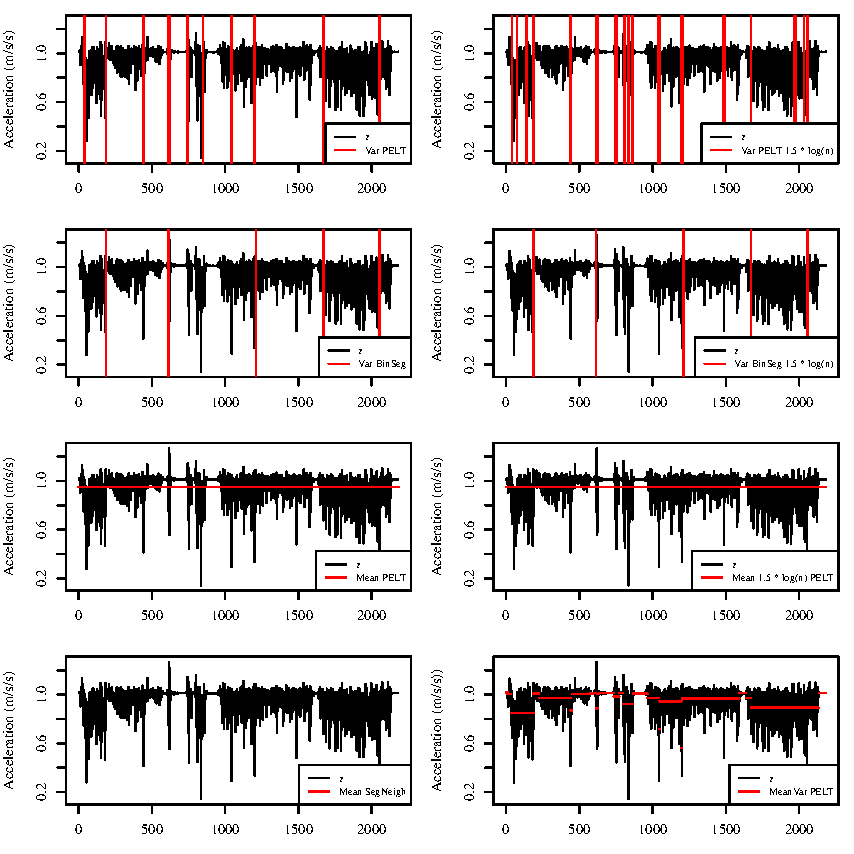
\includegraphics[width=\textwidth]{img/R_comparisonMethodsZ.pdf}
\centering
\caption{Comparison different algorithms for change point detection \newline in accelerometer z-axis output\label{cpcomp}}
\end{figure} 


The next sections show the change points detected for average height, average speed, average slope, and variance of the total acceleration for all the measured routes. The change points are assigned a location through linking its time stamp with the time of the GPS data. 

\clearpage

\subsection{Change point and Segments found for the Meetrollator walking route}
In figure \ref{routeM} the route of the measurement rollator is shown with the detected change points indicated. The numbers show the time index which is the same as found in the graph \ref{routeR}, which shows the datasets with the changepoints and segments. The average walking speed was 1.2$m/s$. 

\begin{figure}[ht]
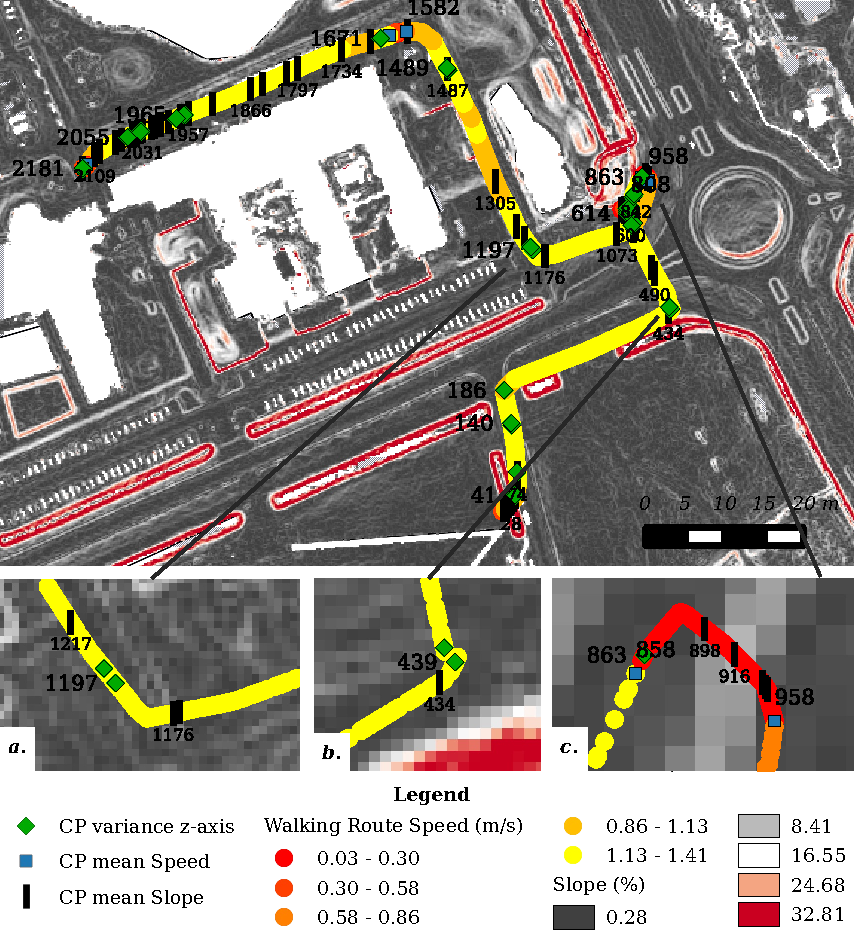
\includegraphics[width=\textwidth]{img/R_meetrollatorroute.pdf}
\centering
\caption{Change points for the Meet Rollator route\label{routeM}}
\end{figure} 

\clearpage

The right zoomed in square shows the area where a little detour was taken, walking down and up the curb again. The slope map clearly shows the location of the curb and the pavement. Specifically in the top, the crosses show a decrease and increase in speed while going over the curb. The red dots show a change in slope where the curb is located. Only no change in variance is detected. The left zoomed in square shows again that the change point in slope is detected, where the little red dots and the slope map show a bump. Though the change point in the accelerometer fall slightly later in the route. 
The slope is derived from the location of the track, while the accelerometer is linked to the time stamp of the GPS. Because of GPS inaccuracy's these points do not have to fall at the same point in the route.

\begin{figure}[hb]
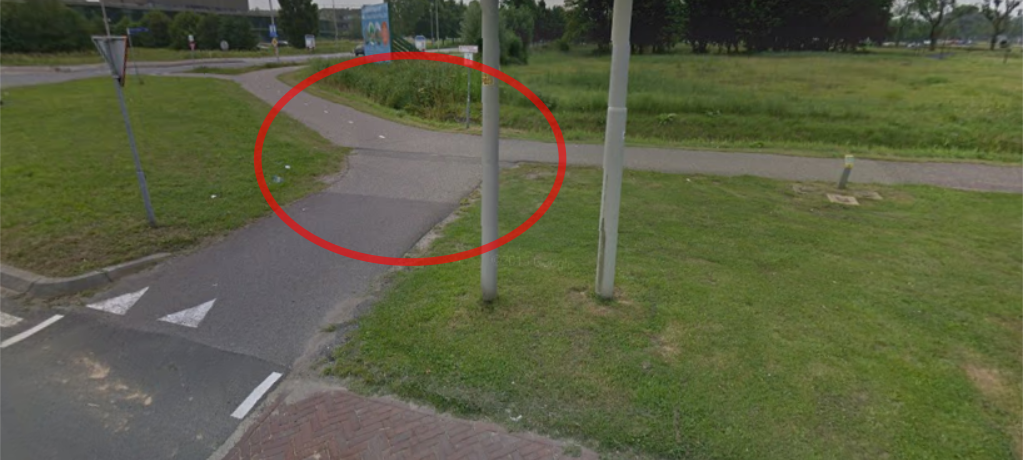
\includegraphics[ width=\textwidth]{img/R_bochtwageningenmeetrollator3.png}
\centering
\caption{ Example surface of Detail B. from figure \ref{routeM} \label{straatbocht}}
\end{figure} 

\renewcommand{\arraystretch}{1}

\begin{table}[hb]
\centering
\caption{Summary of changepoint output and methods used, per dataset, for the MeetRollator walking route}
\label{}
\begin{tabular}{|p{70pt}|p{70pt}|p{70pt}|p{70pt}|p{70pt}|}
\hline
& Slope & Speed & Variance z-axis & Variance total \newline acceleration\\
\hline 
Changepoint type   	& Change in mean 	& Change in mean 	& Change in variance 		& Change in variance \\
Method of analysis	& PELT 				& PELT 				& PELT 						& PELT \\
Test Statistic 		& Normal 			& Normal 			& Normal 					& Normal \\
Type of penalty		& Manual with value \newline 11.53131   & Manual with value\newline 11.53131  & Manual with value\newline 11.53131 & MBIC with value\newline 23.06262 \\
Minimum Segment Length	& 1 			& 1 				& 2 						& 2 \\
Maximum no. \newline of cpts 	&  Inf 			&  Inf  			& Inf 						& Inf \\
Number of \newline changepoints 	& 69			&  7 				& 28 						& 12 \\
\hline
\multicolumn{5}{|l|}{Created Using changepoint version 2.2 } \\
\hline
\end{tabular}
\end{table}

\clearpage

\begin{figure}[ht]
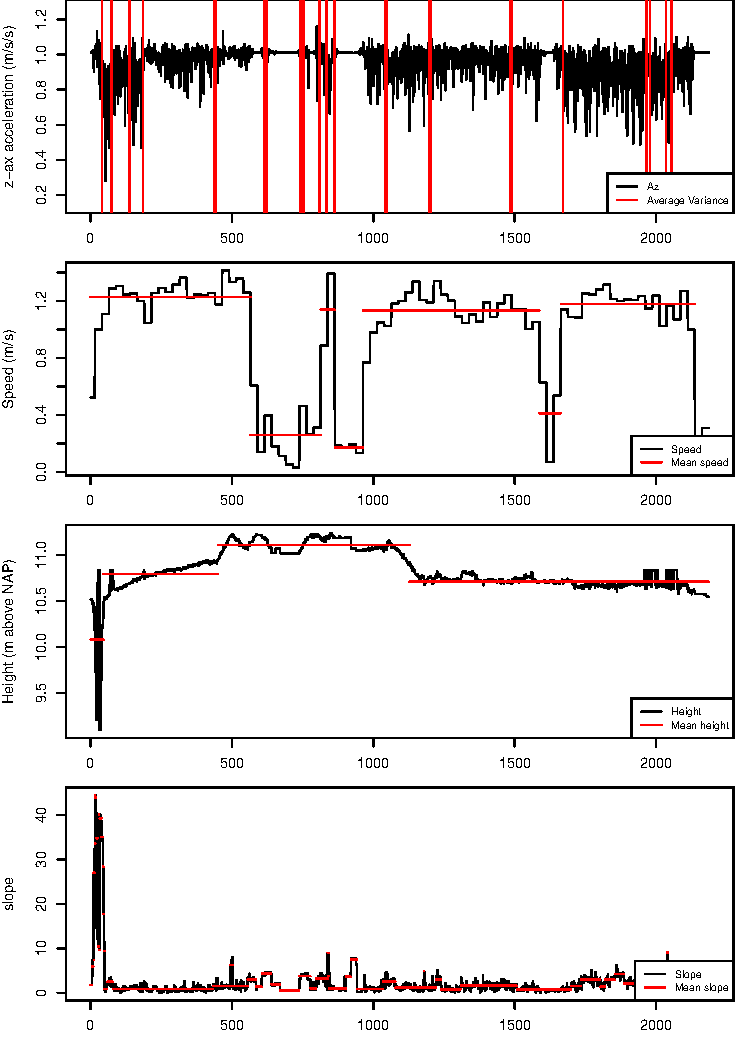
\includegraphics[ width=\textwidth]{img/R_ChangePointComparisonmeetr.pdf}
\centering
\caption{Change point segments, per dataset, for the MeetRollator route\label{routeR}}
\end{figure} 





\clearpage

\subsection{Change point and Segments found for the Leica walking route (without accelerometer)}
From the failed measurements, there was on route walked with a Leica system. Though, there are no accelerometer measurements on this route, the location is more accurate and the comparison with the slope and speed could give better results. 

\begin{figure}[ht]
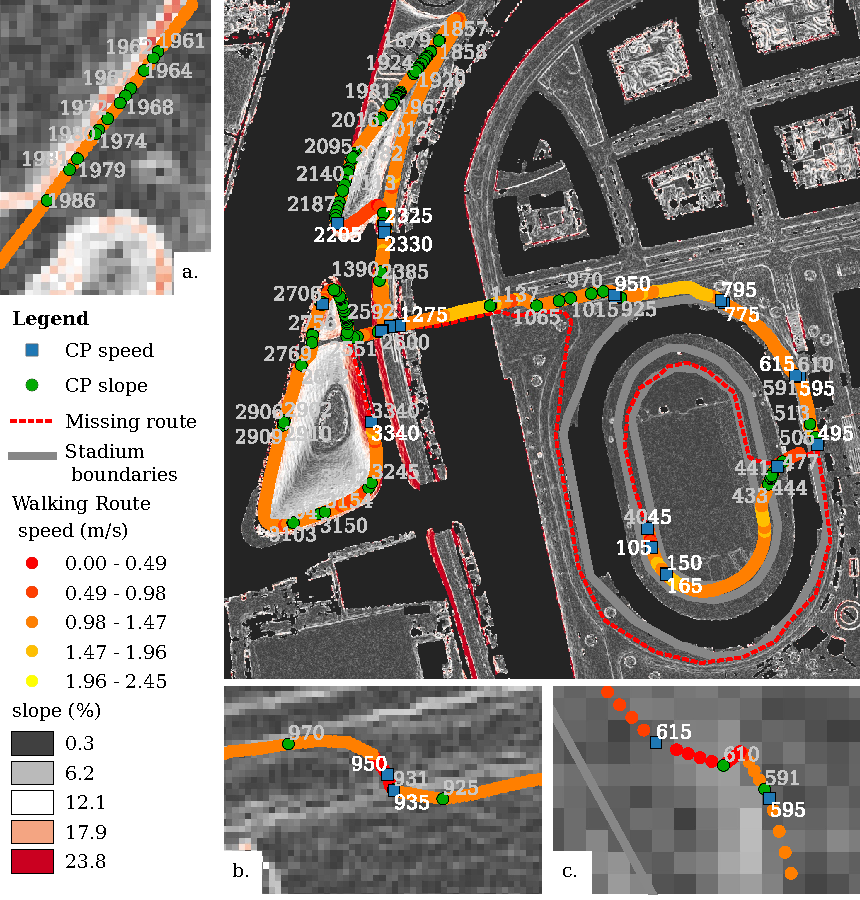
\includegraphics[width=\textwidth]{img/R_leicaroute.pdf}
\centering
\caption{Change points in speed and slope for the Leica route on the map\label{routeLeicaMap}}
\end{figure}

\clearpage

\begin{table}[!ht]
\centering
\caption{summary change point methods for Leica}
\label{leicaCP}
\begin{tabular}{|p{175.3pt}|p{100.3pt}|p{100.3pt}|}
\hline
.. & Slope & Speed \\
\hline 
Change point type   	& Change in mean 	& Change in mean 	\\
Method of analysis	& PELT 				& PELT 				\\
Test Statistic 		& Normal 			& Normal 			\\
Type of penalty		&  MBIC with value, 24.34118  & AIC with value, 4  \\
Minimum Segment Length	& 1 			& 1 				 \\
Maximum no. of cpts 	&  Inf 			&  Inf  			 \\
Number of changepoints 	& 123			&  20				 \\
\hline
\multicolumn{3}{|l|}{Created Using changepoint version 2.2 } \\
\hline
\end{tabular}
\end{table}

% Section about changepoint method Leica route, without Accelerometer
\begin{figure}[!hb]
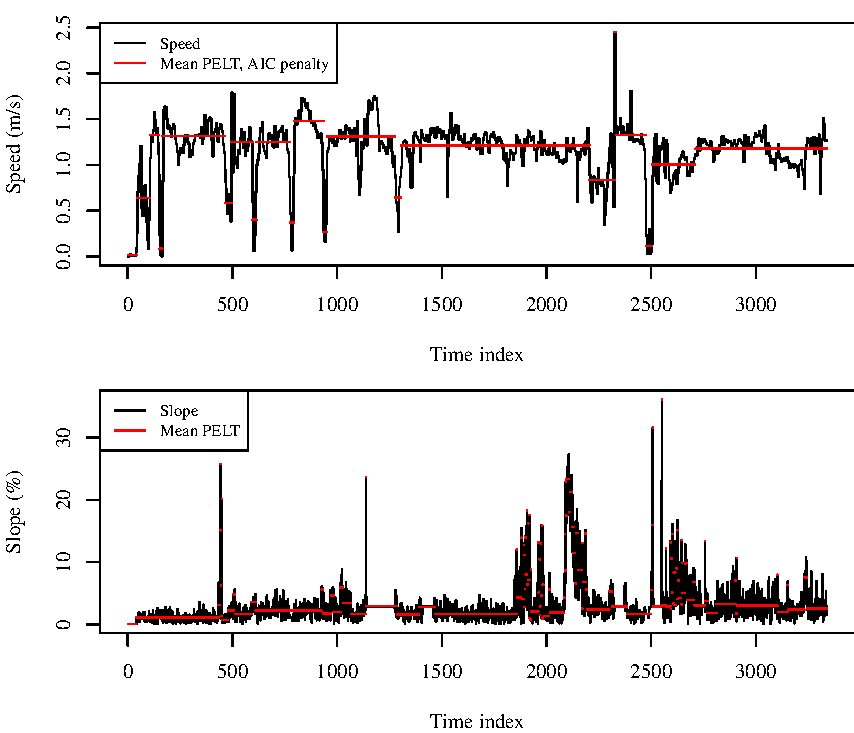
\includegraphics[width=\textwidth]{img/R_comparisonMethodsLeica.pdf}
\centering
\caption{Change point segments in speed and slope for the Leica route\label{routeLeica}}
\end{figure} 


\clearpage

%Bike route
\subsection{Change point and Segments found for the bike route}
For testing the accelerometer application, a route with GPS and the accelerometer app was conducted on the bike. This resulted into the following data. Figure \ref{routeB2} shows the route with the bike. The left zoom square shows a right crossroad, where the bike path is interrupted by another type of road. Going from concrete to tiled paving. See figure \ref{crossroad} showing a Google street-view of the bicycle lane changing to tiles at the crossing. The middle square shows a stop with the bike, before crossing the road. Here all indicators show a change point. The speed, slope, and acceleration in vertical direction. The right square shows a street with speed bumps that have to be crossed with the bike as well. The slope change points, indicate roughly these bumps, though they do not show in any other parameter. 

\begin{figure}[hb]
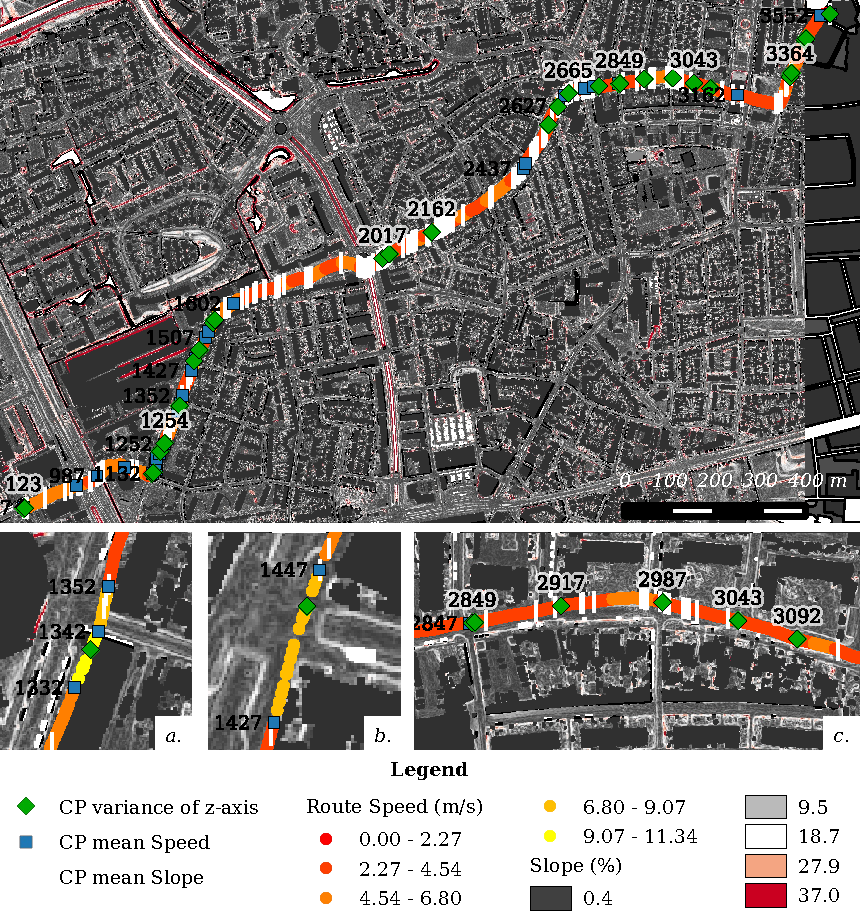
\includegraphics[width=\textwidth]{img/R_Bikeroute.pdf}
\centering
\caption{Change points for the Bike route\label{routeB2}}
\end{figure} 

\clearpage

\begin{figure}[!ht]
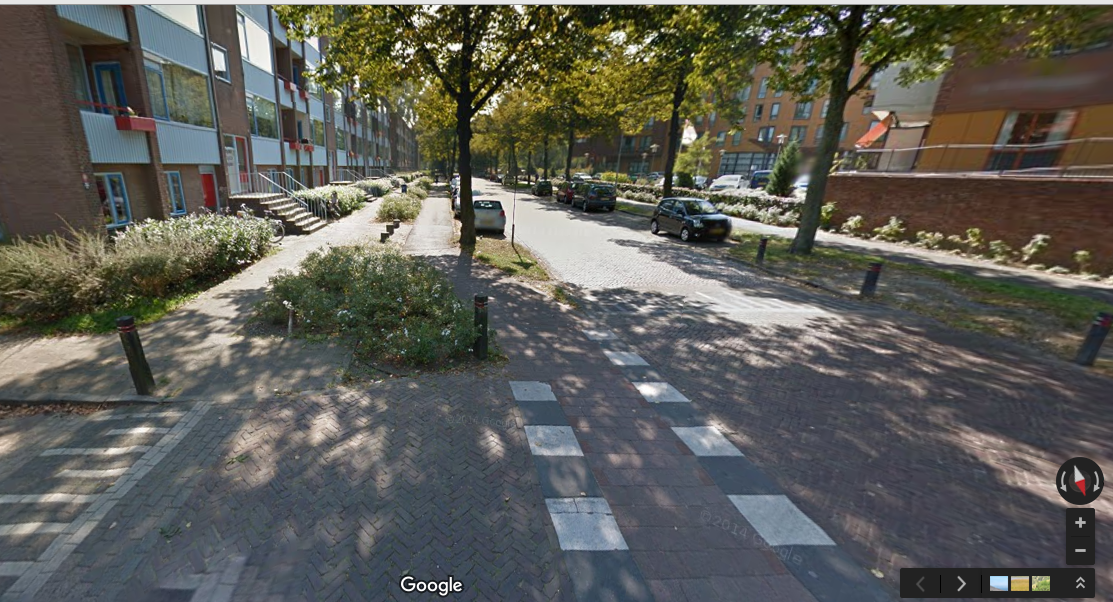
\includegraphics[width=\textwidth]{img/R_crossroad.png}
\centering
\caption{Google street-view of cross road, bicycle lane change. \label{crossroad}}
\end{figure} 

\begin{table}[!hb]
\centering
\caption{Summary}
\label{sss}
\begin{tabular}{|p{109pt}|p{85pt}|p{85pt}|p{85pt}|}
	\hline
	.. & Slope & Speed & Variance z-axis \\
	\hline 
	Changepoint type   	& Change in mean 	& Change in mean 	& Change in variance \\
	Method of analysis	& PELT 				& PELT 				& PELT\\
	Test Statistic 		& Normal 			& Normal 			& Normal\\
	Type of penalty		&  MBIC with value, 24.5802  & Manual with value, 12.2901 & Manual with value, 12.2901\\
	Minimum Segment Length	& 1 			& 1 				& 2 \\
	Maximum no. of cpts 	&  Inf 			&  Inf  			& Inf \\
	Number of changepoints 	& 195			&  27 				& 32 \\
	\hline
	\multicolumn{4}{|l|}{Created Using changepoint version 2.2 } \\
	\hline
\end{tabular}
\end{table}
\clearpage

\begin{figure}[ht]
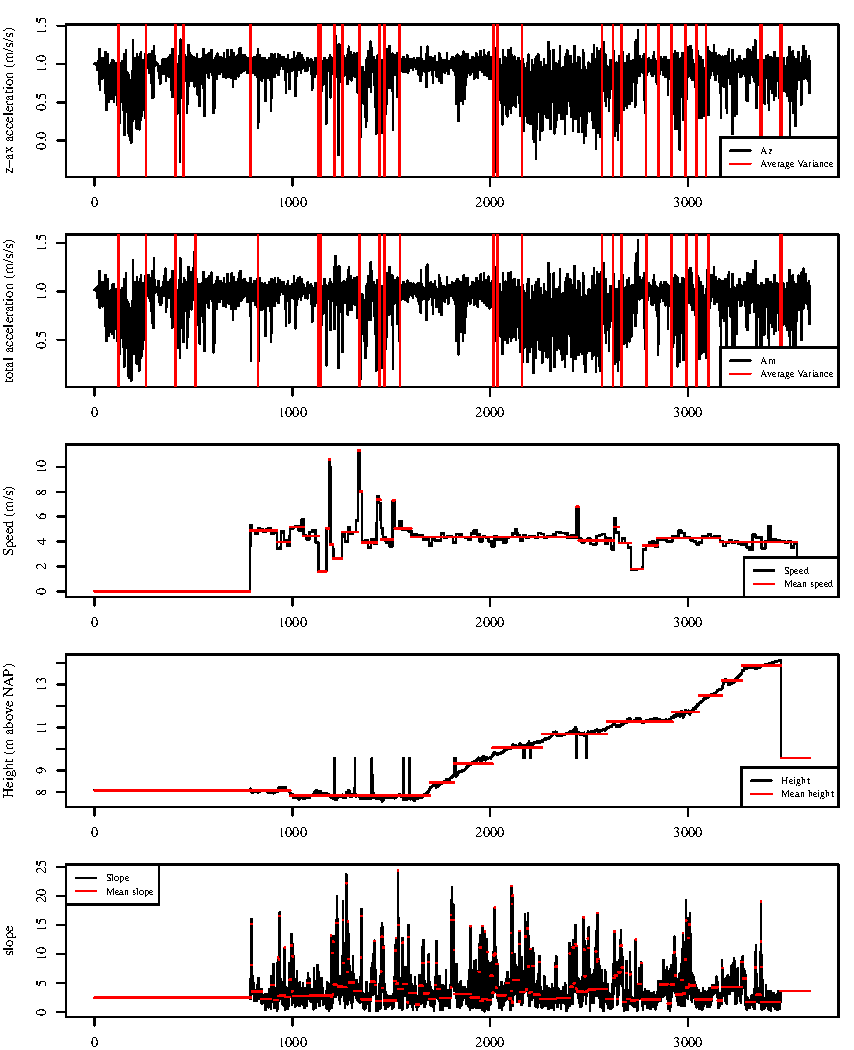
\includegraphics[ width=\textwidth]{img/R_ChangePointComparisonbike.pdf}
\centering
\caption{Change point segments for the Bike route\label{routeB}}
\end{figure} 



\clearpage